
\section{Approach} \label{sec:approach}
Our general approach to the discourse structure identification task involves two steps. First, we perform sequence labeling by training the models to make a binary classification, assigning one of two labels to each of the input tokens. In the NeurIPS task, we label each token as \texttt{Is-abstract} or \texttt{Is-body}. In the Podcast task, we label each token as \texttt{Is-intro} or \texttt{Not-intro}. We then use a boundary detector based on a maximum difference algorithm to identify the best split position(s) (see below). Each of our models has a different approach to the first part, while the algorithm for the second task is consistent across the board.

To fine-tune BERT, we first tokenize the documents using BERT's tokenizer. If a document is longer than 512 tokens, we segment it into overlapping spans because of BERT's input length limit. Following the practice in \citet{devlin2018bert}, We use a sequence length of 512 with 128 overlapping tokens between spans. The spans are re-merged after training using a maximum minimum method described in \citet{devlin2018bert}. 

\begin{figure*}
    \centering
    \begin{subfigure}[h]{0.8\textwidth}
        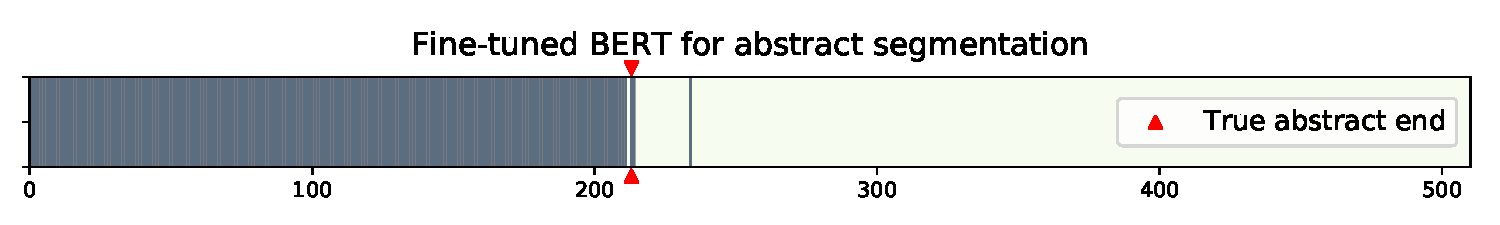
\includegraphics[width=\textwidth]{score_dist_bert_abstract.pdf}
        \vspace{-0.3in}
        \caption{}
        % \caption{Example where the fine-tuned BERT's predicted scores align well with the ground truth.}
        \label{fig:score_dist_bert_abstract}
    \end{subfigure}
    \begin{subfigure}[h]{0.8\textwidth}
        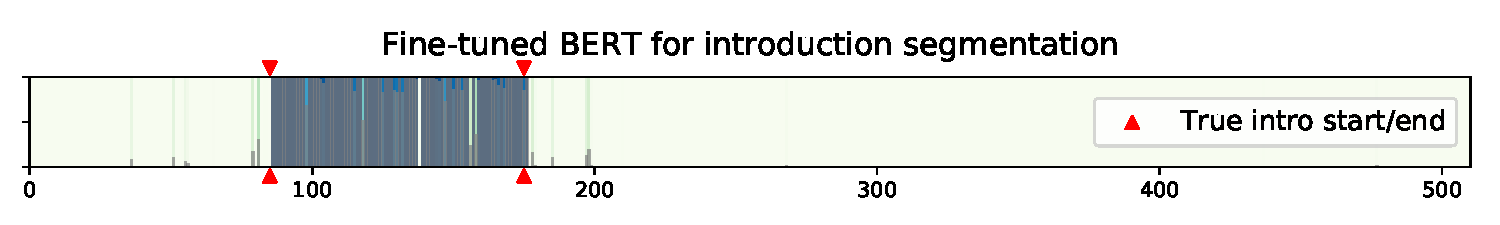
\includegraphics[width=\textwidth]{score_dist_bert_intro.pdf}
        \vspace{-0.3in}
        \caption{}
        \label{fig:score_dist_bert_intro}
    \end{subfigure}
    \begin{subfigure}[h]{0.8\textwidth}
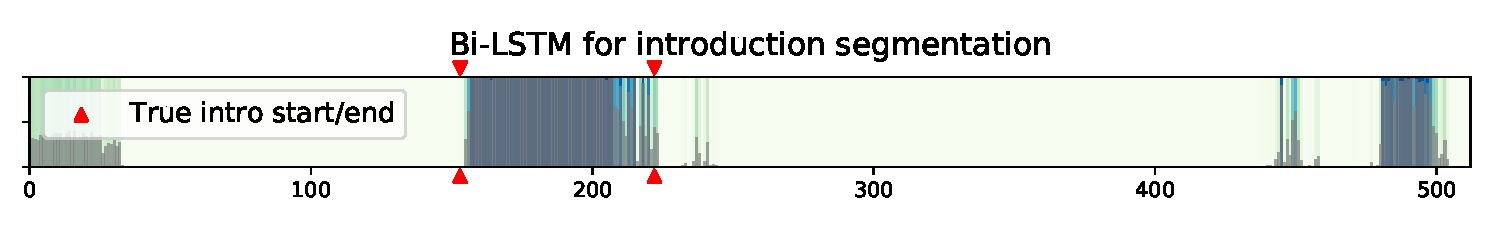
\includegraphics[width=\textwidth]{score_dist_Bi-LSTM.pdf}
        \vspace{-0.3in}
        \caption{}
        % \caption{Example where the Bi-LSTM mistakenly identifies another block of text as introduction.}
        \label{fig:score_dist_lstm}
    \end{subfigure}
    \begin{subfigure}[b]{0.8\textwidth}
        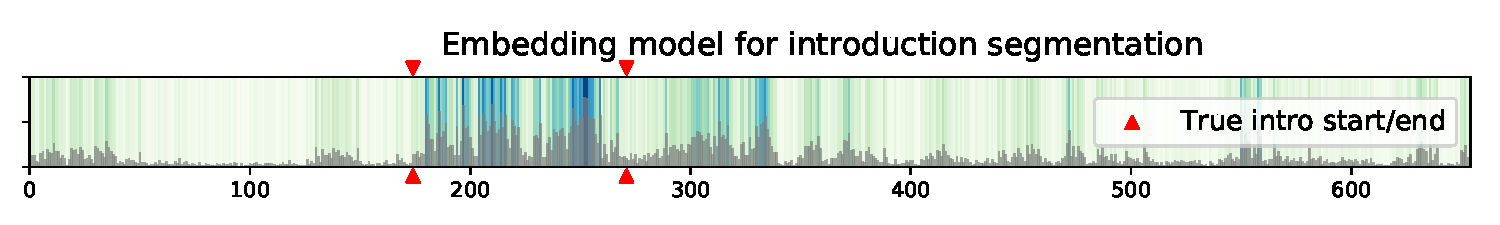
\includegraphics[width=\textwidth]{score_dist_Embedding.pdf}
        \vspace{-0.3in}
        \caption{}
        % \caption{Example where the embedding model correctly identifies the introduction, but also predicts other parts of the document as high Is-intro texts.}
        \label{fig:score_dist_embedding}
    \end{subfigure}
    \caption{Distribution of the models' prediction scores. the x-axis are the index of tokens. Each vertical line is the probability for being \texttt{Is-intro} or \texttt{Is-abstract} for a token. The darker lines indicate higher probabilities, while the gray bars show the raw probability scores. The ground truth boundaries are indicated.}\label{fig:score_dist}
\end{figure*}


We use the pre-trained BERT model \texttt{bert-base-uncased} provided in the \texttt{PyTorch Transformers} package \cite{Wolf2019HuggingFacesTS}. We train the model for 300 epochs, using the \texttt{AdamW} optimizer with an initial learning rate of $2e-5$. Linear warm-up and decay are used for learning rate adjustment. The cross entropy function is used as the loss function.

The RNN model uses a similar preprocessing and training strategy. We use a Bi-LSTM model with 64 hidden LSTM units on each direction. Inputs are first passed through a pre-trained embedding layer of GloVe vectors \cite{pennington2014glove}, and then the LSTM layer. We use the \texttt{AdamW} optimizer and learning rate $0.005$, as well as the cross entropy loss function.

For the embedding-based baseline, we extract the word embeddings using the same pretrained BERT model. The sum of the last 4 hidden layers are used to obtain word embeddings for each token in the training and test sets, following a practice in \cite{devlin2018bert}.  We then train a logistic classifier to label each token.

Our models label each token based on a predicted probability score between $0$ and $1$. As a result, the tokens predicted with high \texttt{Is-intro} or \texttt{Is-abstract} probabilities may be found throughout a document (see Figure \ref{fig:score_dist}). We therefore create a simple maximum difference algorithm to identify the best segmentation boundaries. For example, we evaluate how likely each token is the introduction's start position by looking at the tokens before and after it:

\begin{equation}
P_i = \frac{\sum_{n=1}^k{S_{i+n}}}{k} - \frac{\sum_{n=1}^k{S_{i-n}}}{k}
\end{equation}
where $P_i$ is the likelihood for a token to be the start position, $S_i$ is the \texttt{Is-intro} score assigned by our model, and $k$ is a chosen window size. For instance, if $k=20$, for each token $i$, we calculate the average \texttt{Is-intro} score for the 20 tokens before and after $i$. The token $i$ that maximizes $P_i$ is chosen as the introduction start position. We select the introduction end position and the abstract segmentation position in a similar manner.


% The architecture of our model is shown in Figure \ref{fig:model}. 
% \begin{figure*}
%   \centering
%     \includegraphics[width=\textwidth]{bert_model.png}
%       \caption{Model architecture}
%     \label{fig:model}
% \end{figure*}

\begin{figure*}
    \centering
    \begin{subfigure}[h]{0.45\textwidth}
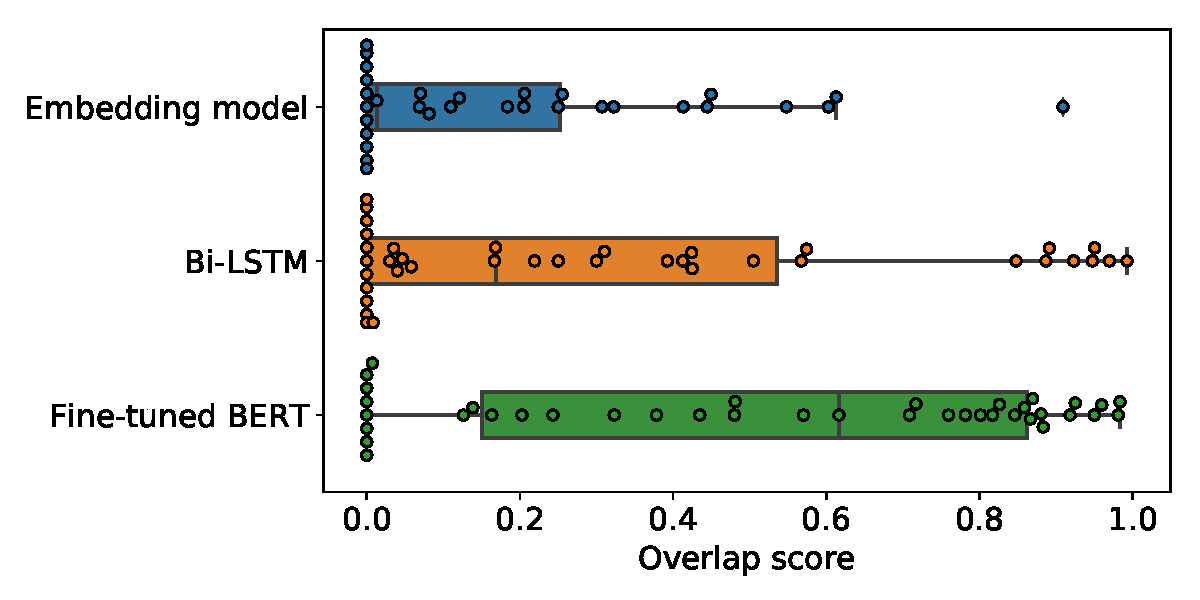
\includegraphics[width=\textwidth]{paper/figs/overlap_swarm_seen.pdf}
        \caption{Test set with seen programs.}
        \label{fig:overlap_seen}
    \end{subfigure}
    \begin{subfigure}[h]{0.45\textwidth}
        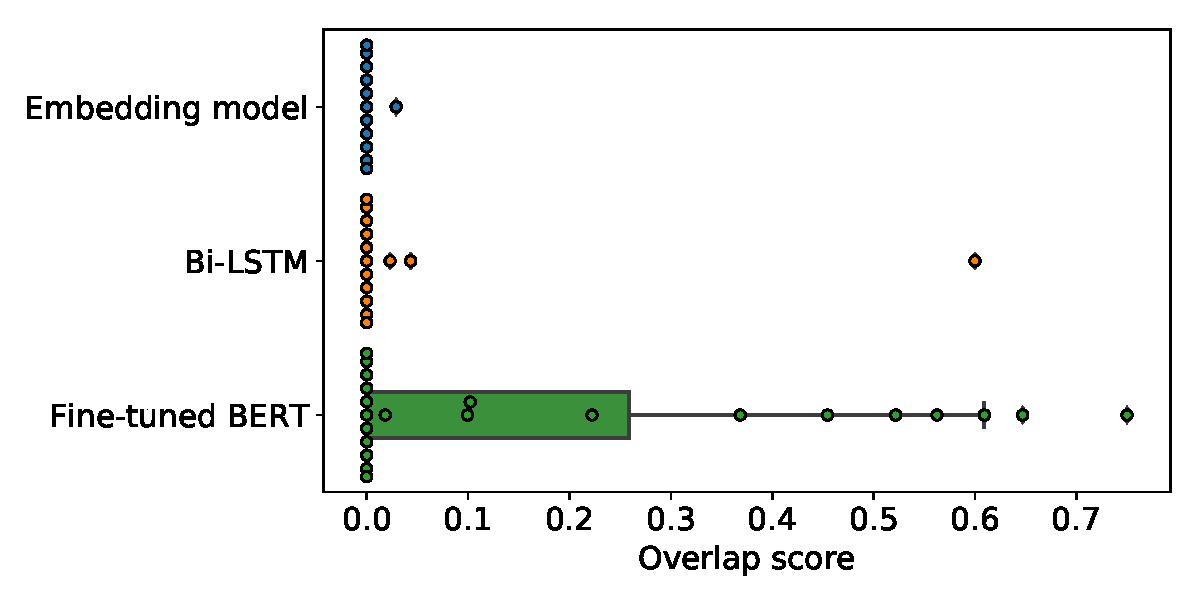
\includegraphics[width=\textwidth]{paper/figs/overlap_swarm_unseen.pdf}
        \caption{Test set with unseen programs.}
        \label{fig:overlap_unseen}
    \end{subfigure}
    \caption{Distribution of overlap scores. The x-axis shows the overlap score between 0 and 1. Each point is a document in the test sets. }\label{fig:overlap_swarm}
\end{figure*}


